
A continuacion se discuten los resultados obtenidos por cada dataset
\begin{figure}[H]
    \centering
        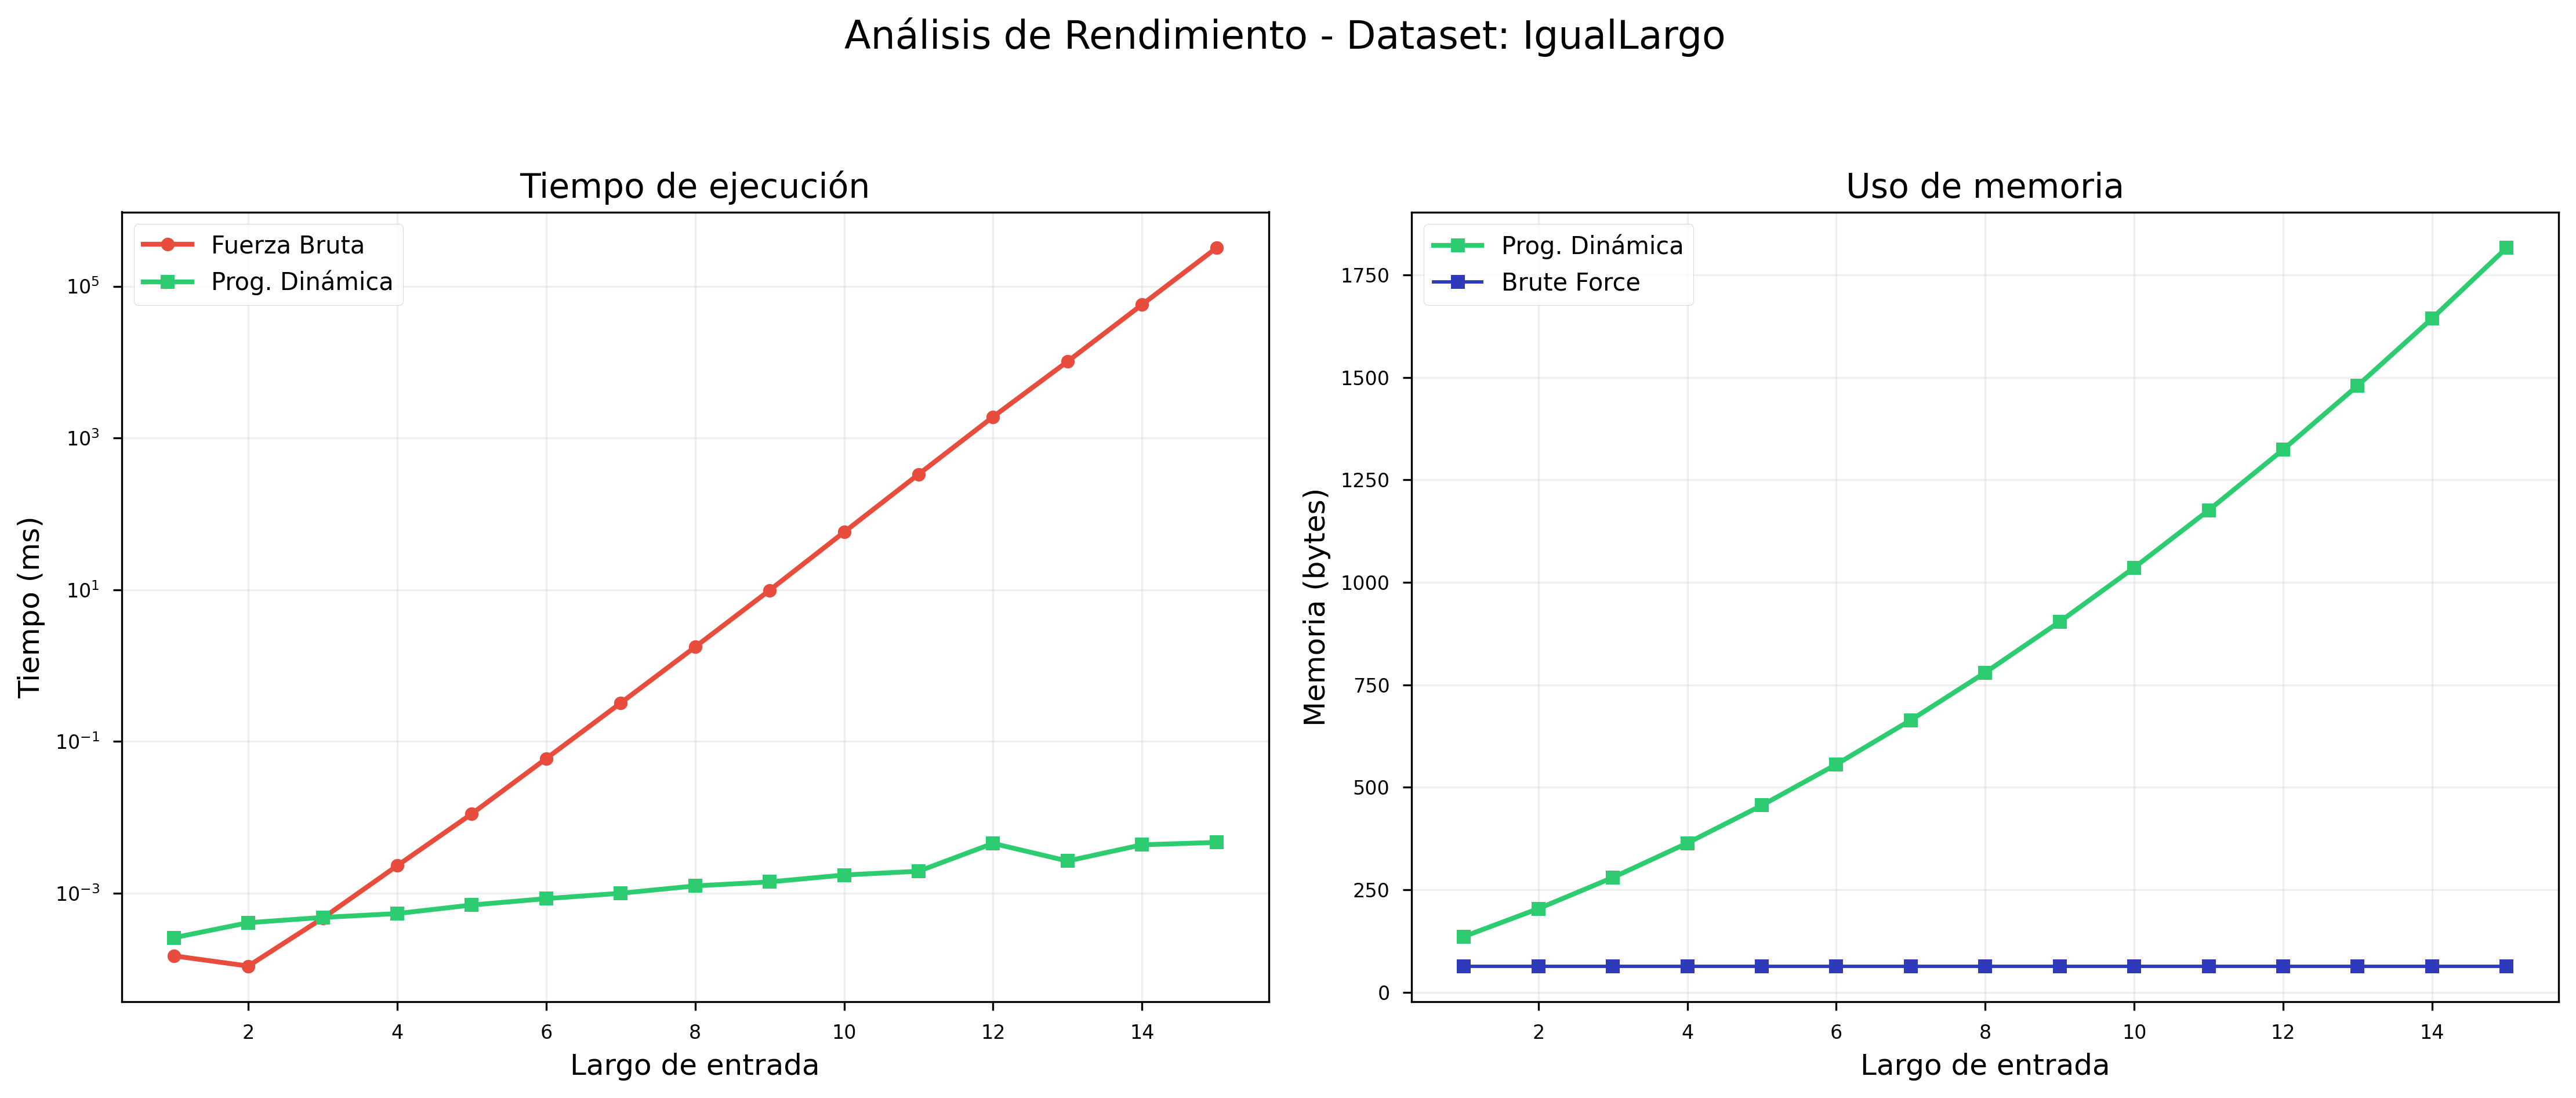
\includegraphics[width=\textwidth]{images/IgualLargo_analisis.png}
    \caption{Cadenas aleatorias de largo creciente}
    \label{fig:scatterplot_1}
\end{figure}
En el grafico de la iquierda se puede observar la inmensa diferencia en tiempo de ejecucion de ambos algoritmos a medida que el tamaño de la entrada crece,
aunque la menor complejidad temporal que maneja programacion dinamica requiere una mayor complejidad espacial.

\begin{figure}[H]
    \centering
        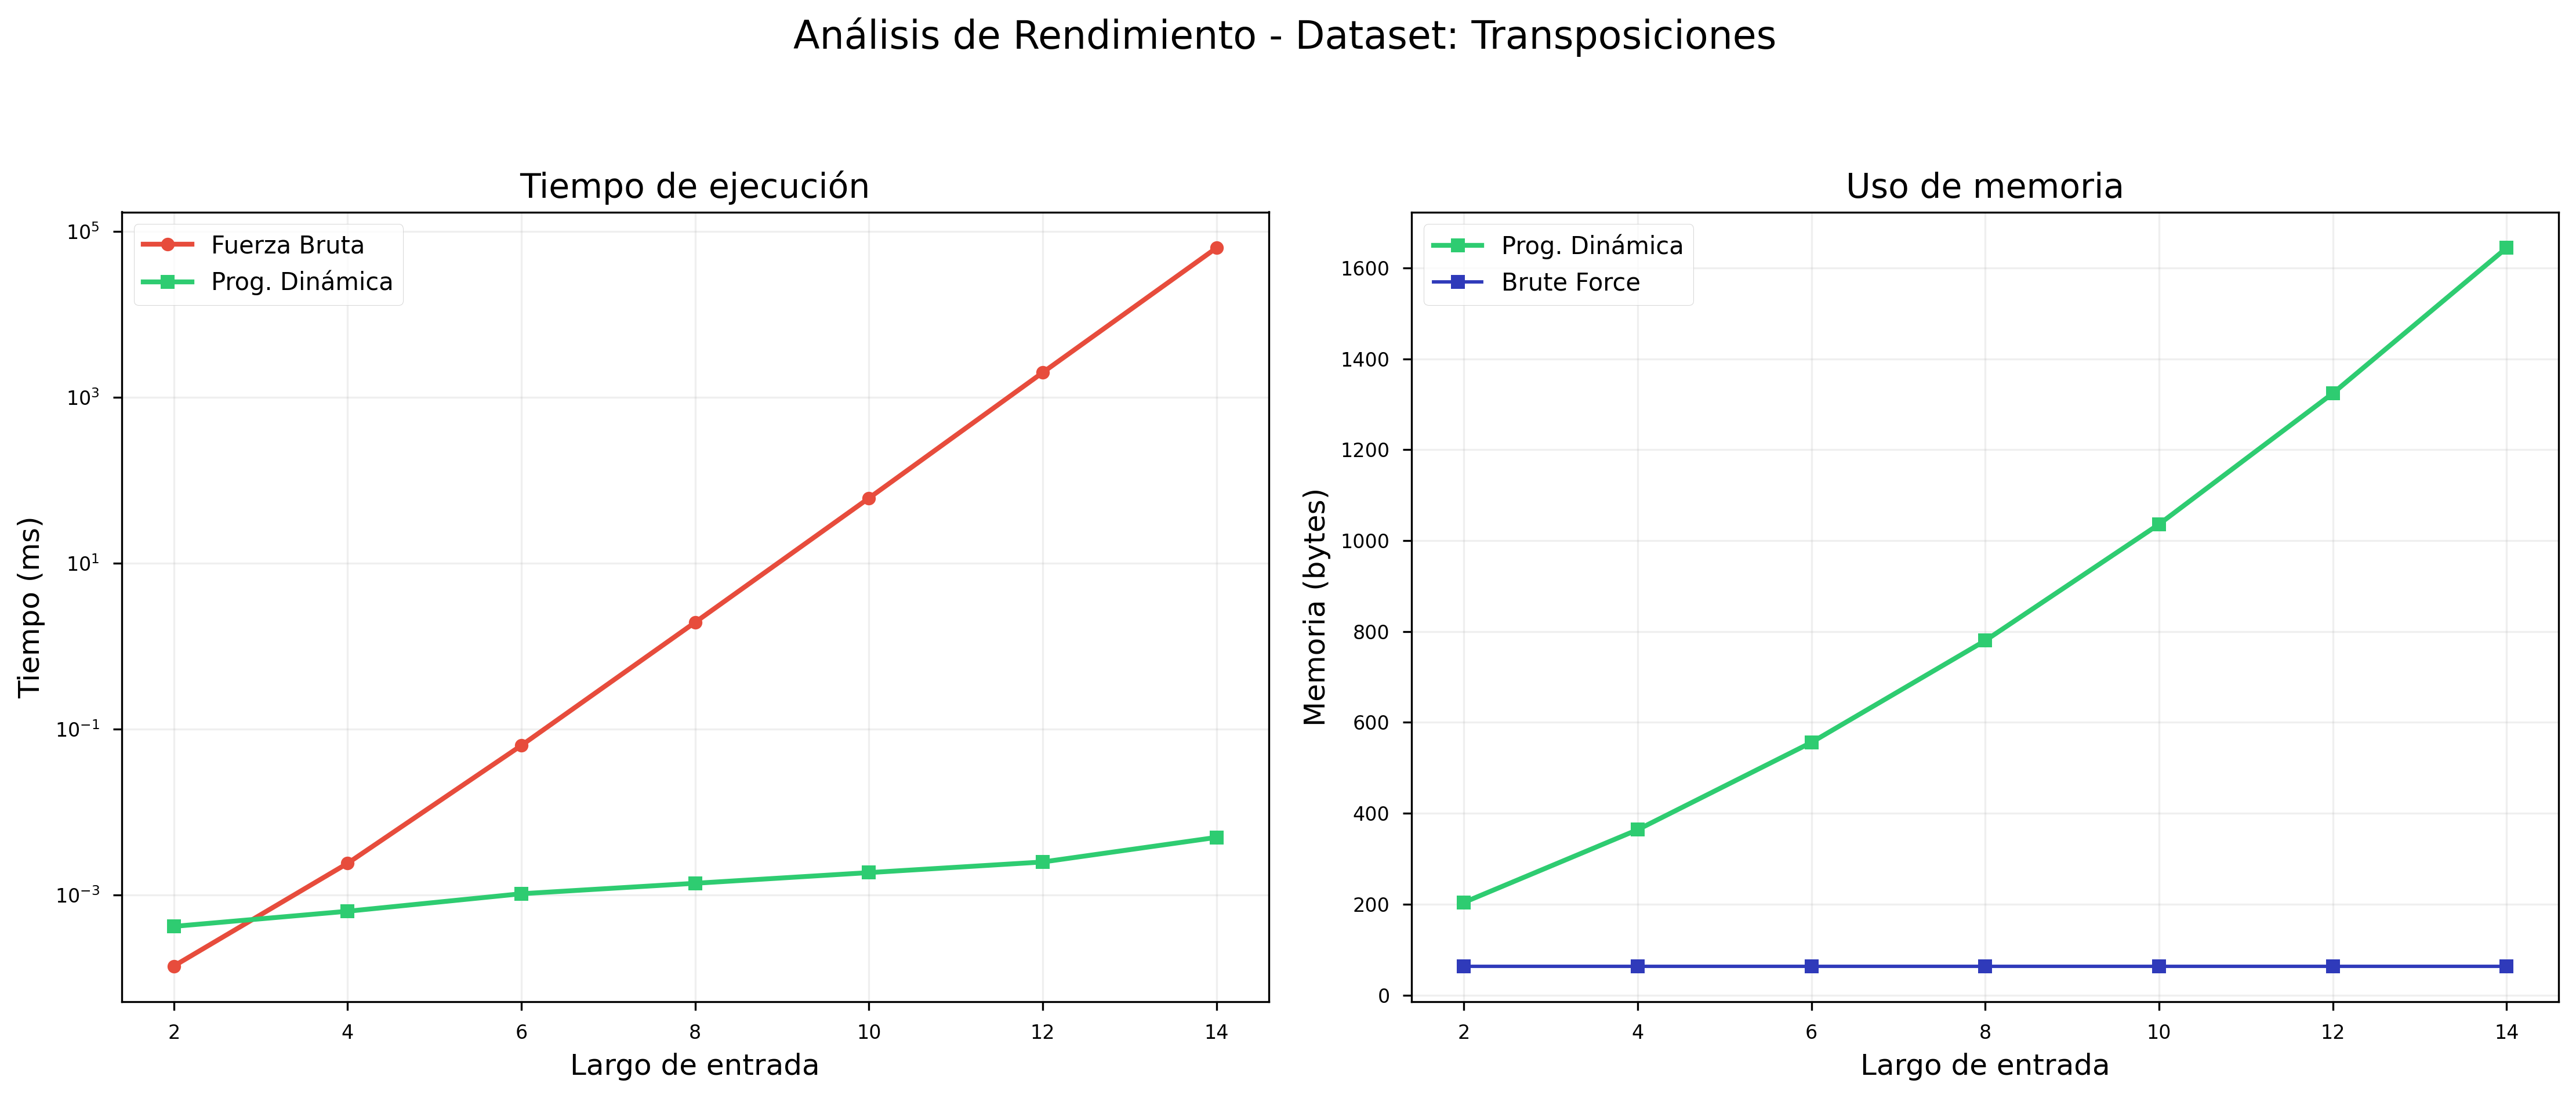
\includegraphics[width=\textwidth]{images/Transposiciones_analisis.png}
    \caption{Cadenas de pares transpuestos}
    \label{fig:scatterplot_2}
\end{figure}
\begin{figure}[H]
    \centering
    \begin{minipage}[t]{0.5\textwidth}
        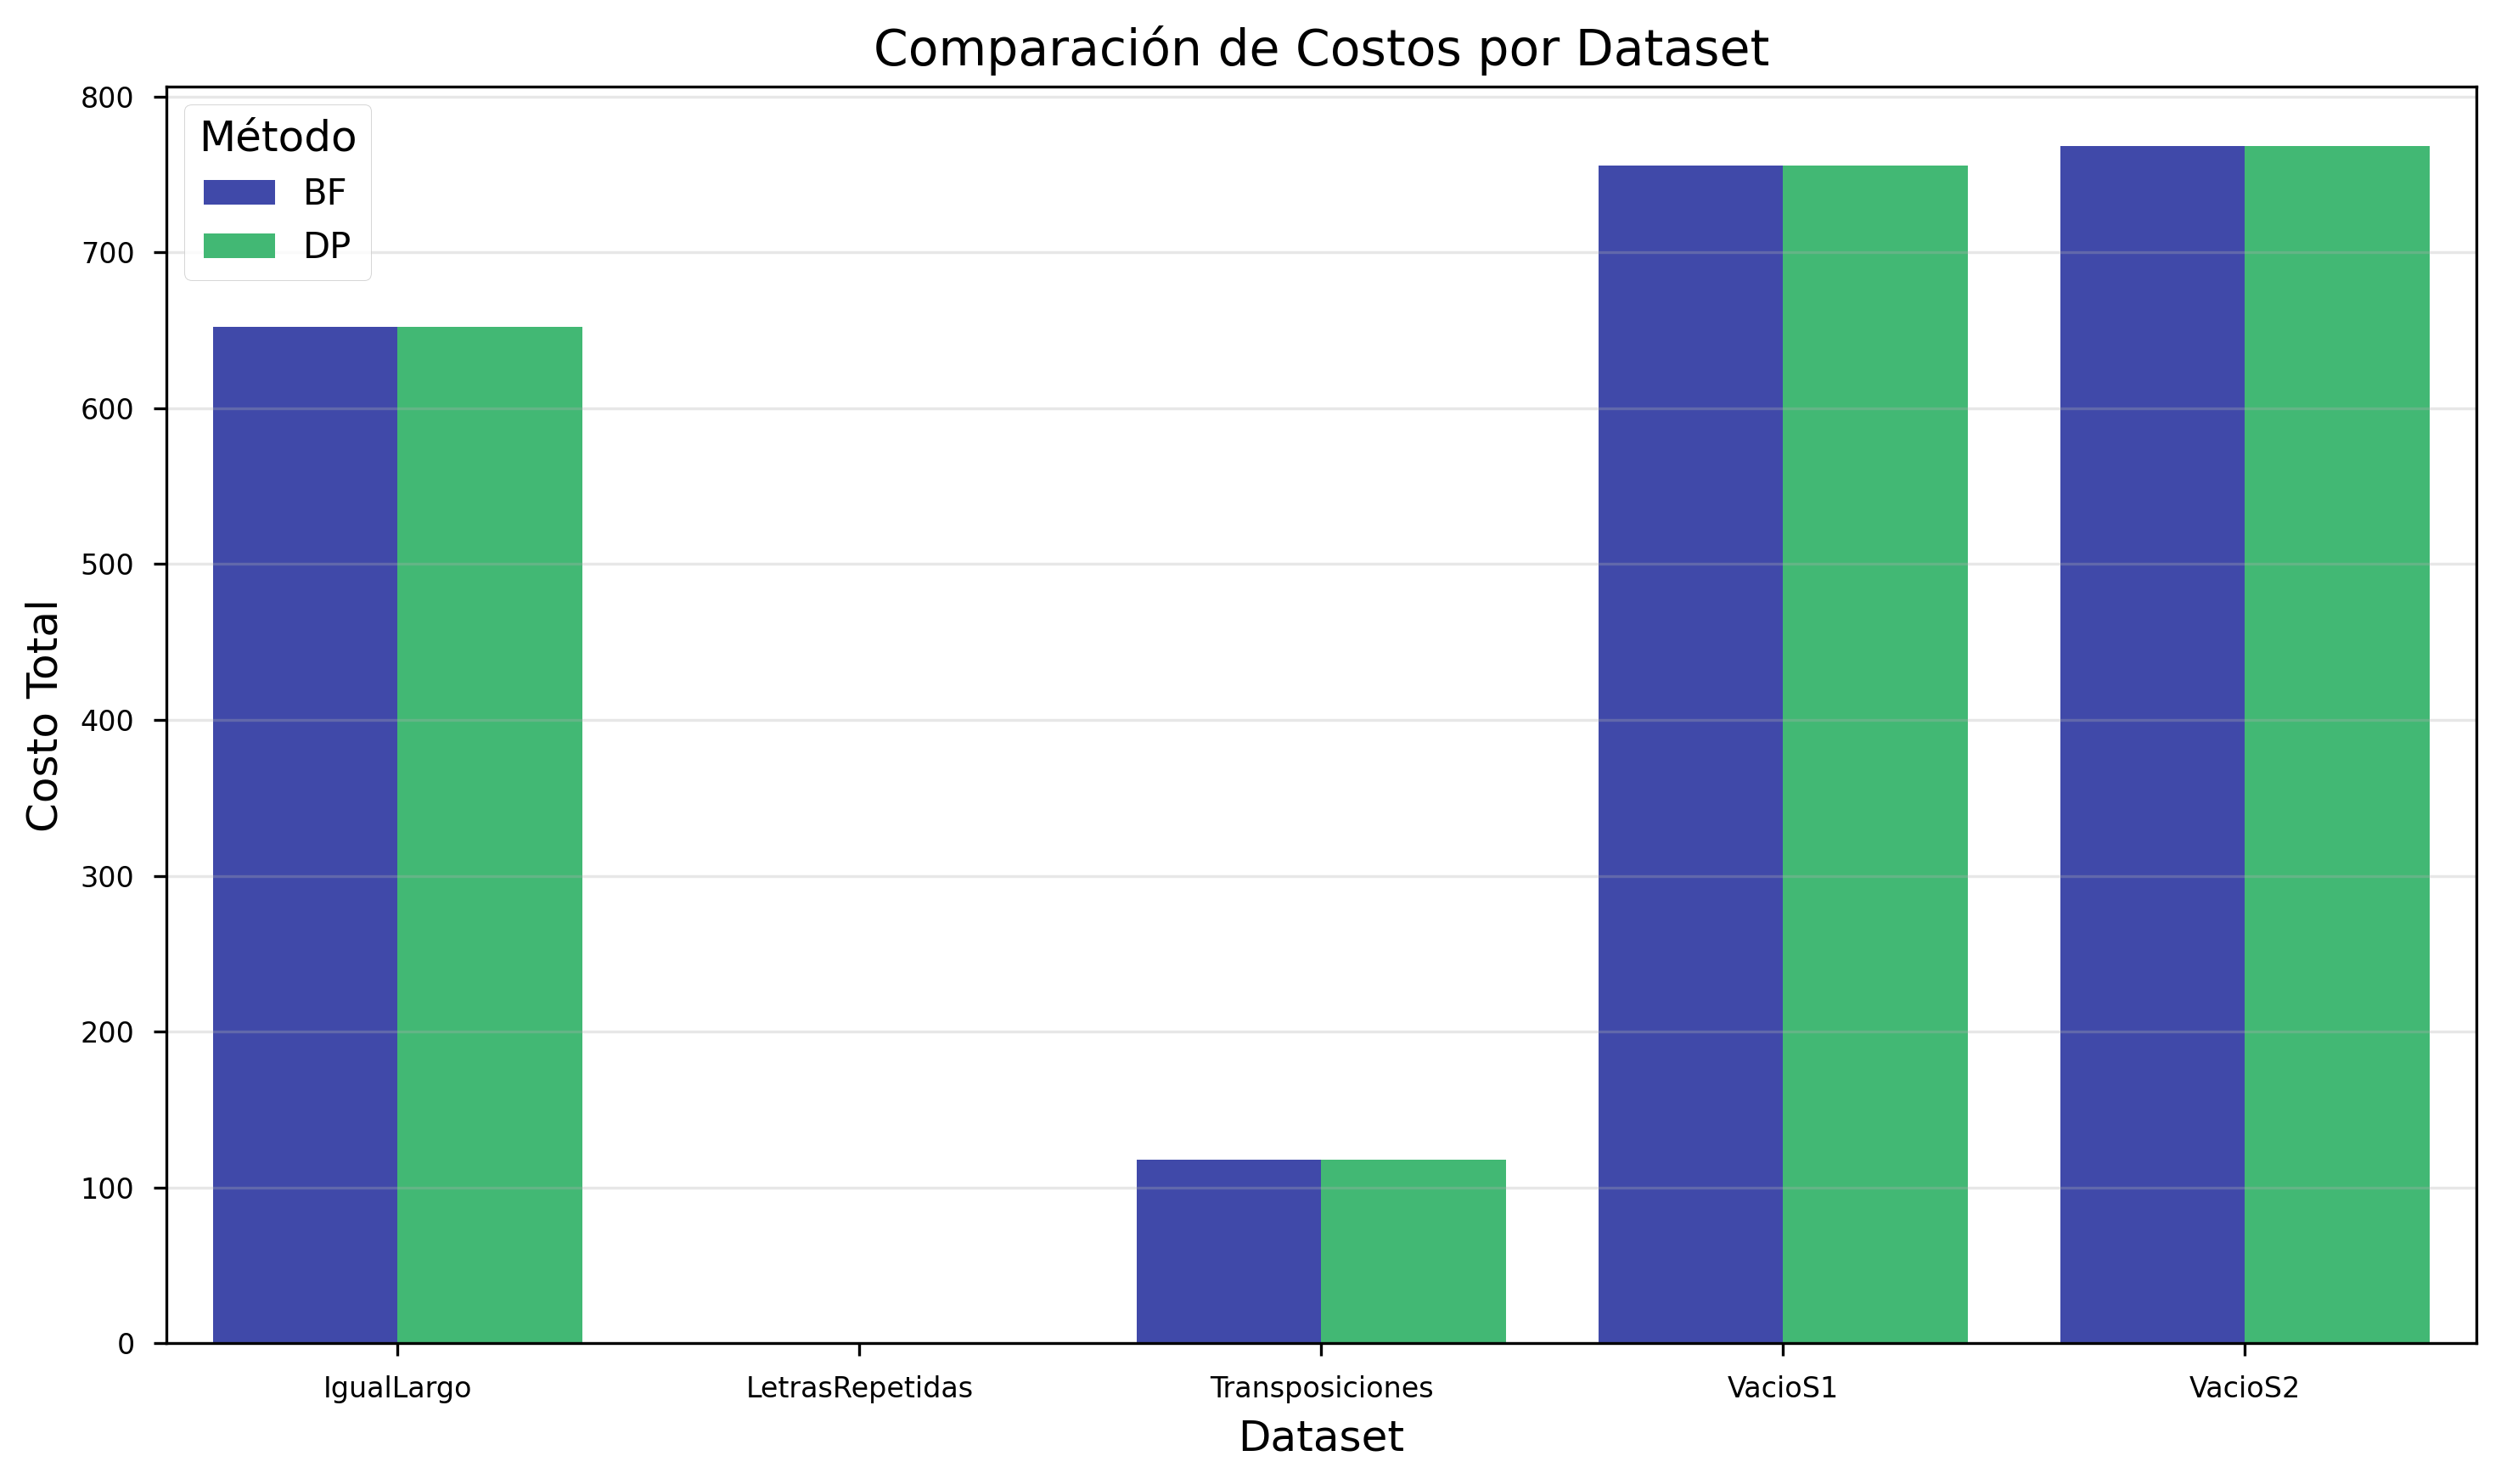
\includegraphics[width=\textwidth]{images/costos_por_dataset.png}
    \end{minipage}%
    \caption{Costos de edicion}
    \label{fig:barplot_1}
\end{figure}
Analizando las figuras 2 y 3 se tiene que las transposiciones juegan un papel relevante puesto que la inclusion de estas aumentan la complejidad, pero esto es por una buena razon,
ya que estas bajan el costo de edicion de las cadenas.

\begin{figure}[H]
    \centering
        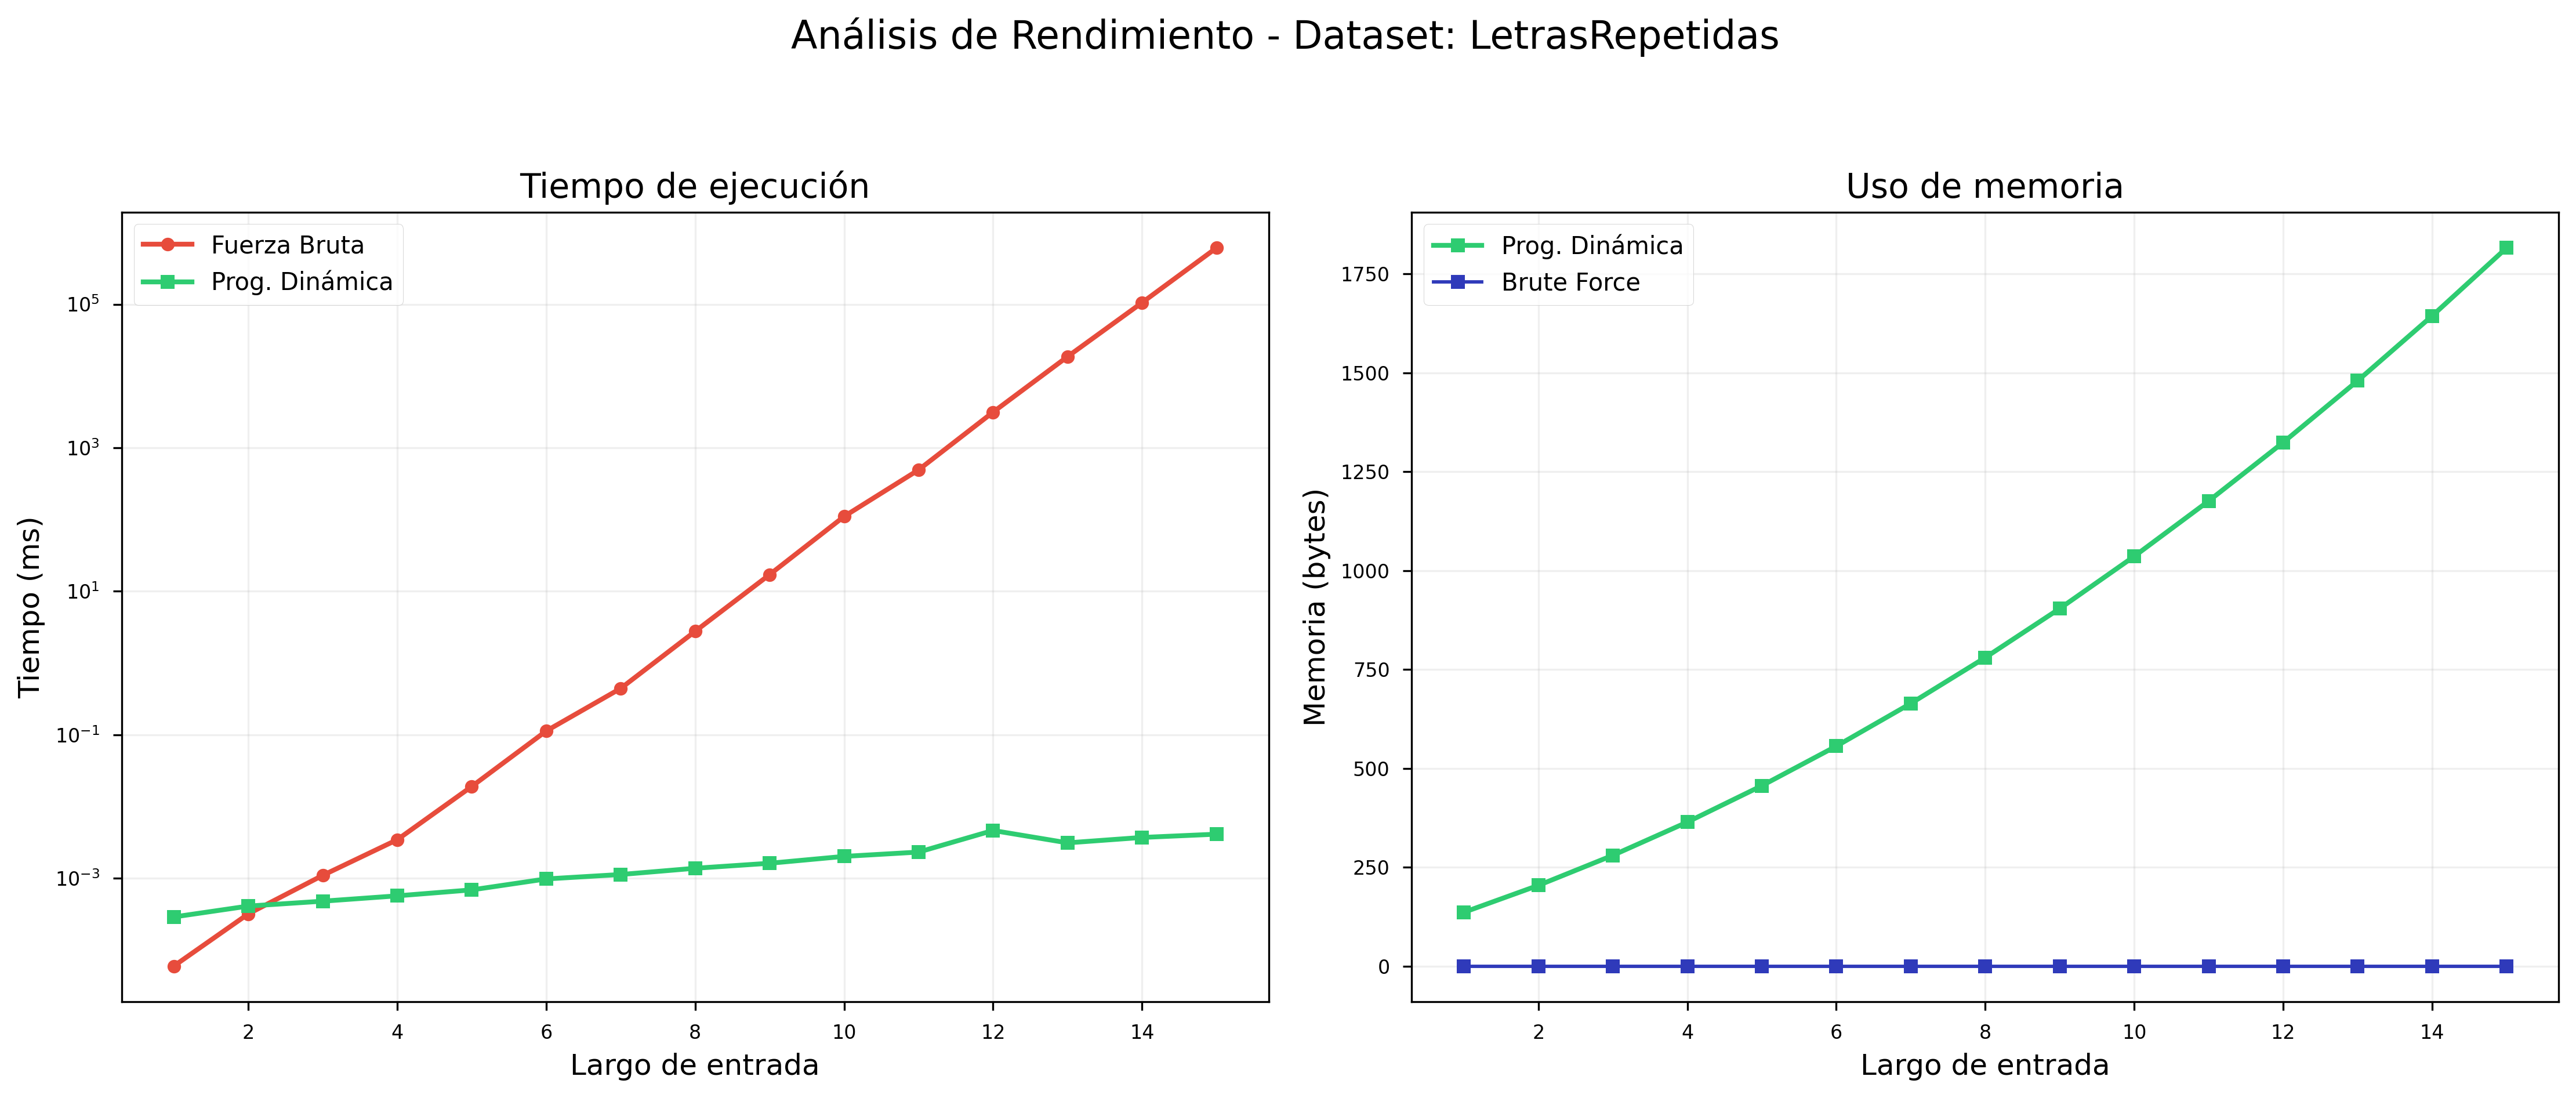
\includegraphics[width=\textwidth]{images/LetrasRepetidas_analisis.png}
    \caption{Cadenas de letras repetidas de largo creciente}
    \label{fig:scatterplot_4}
\end{figure}
Las cadenas repetidas es importante estudiarlas, puesto que estas representan el peor caso en temas de complejidad para fuerza bruta, ya que
las 4 operaciones se realizaran siempre.

\begin{figure}[H]
    \centering
        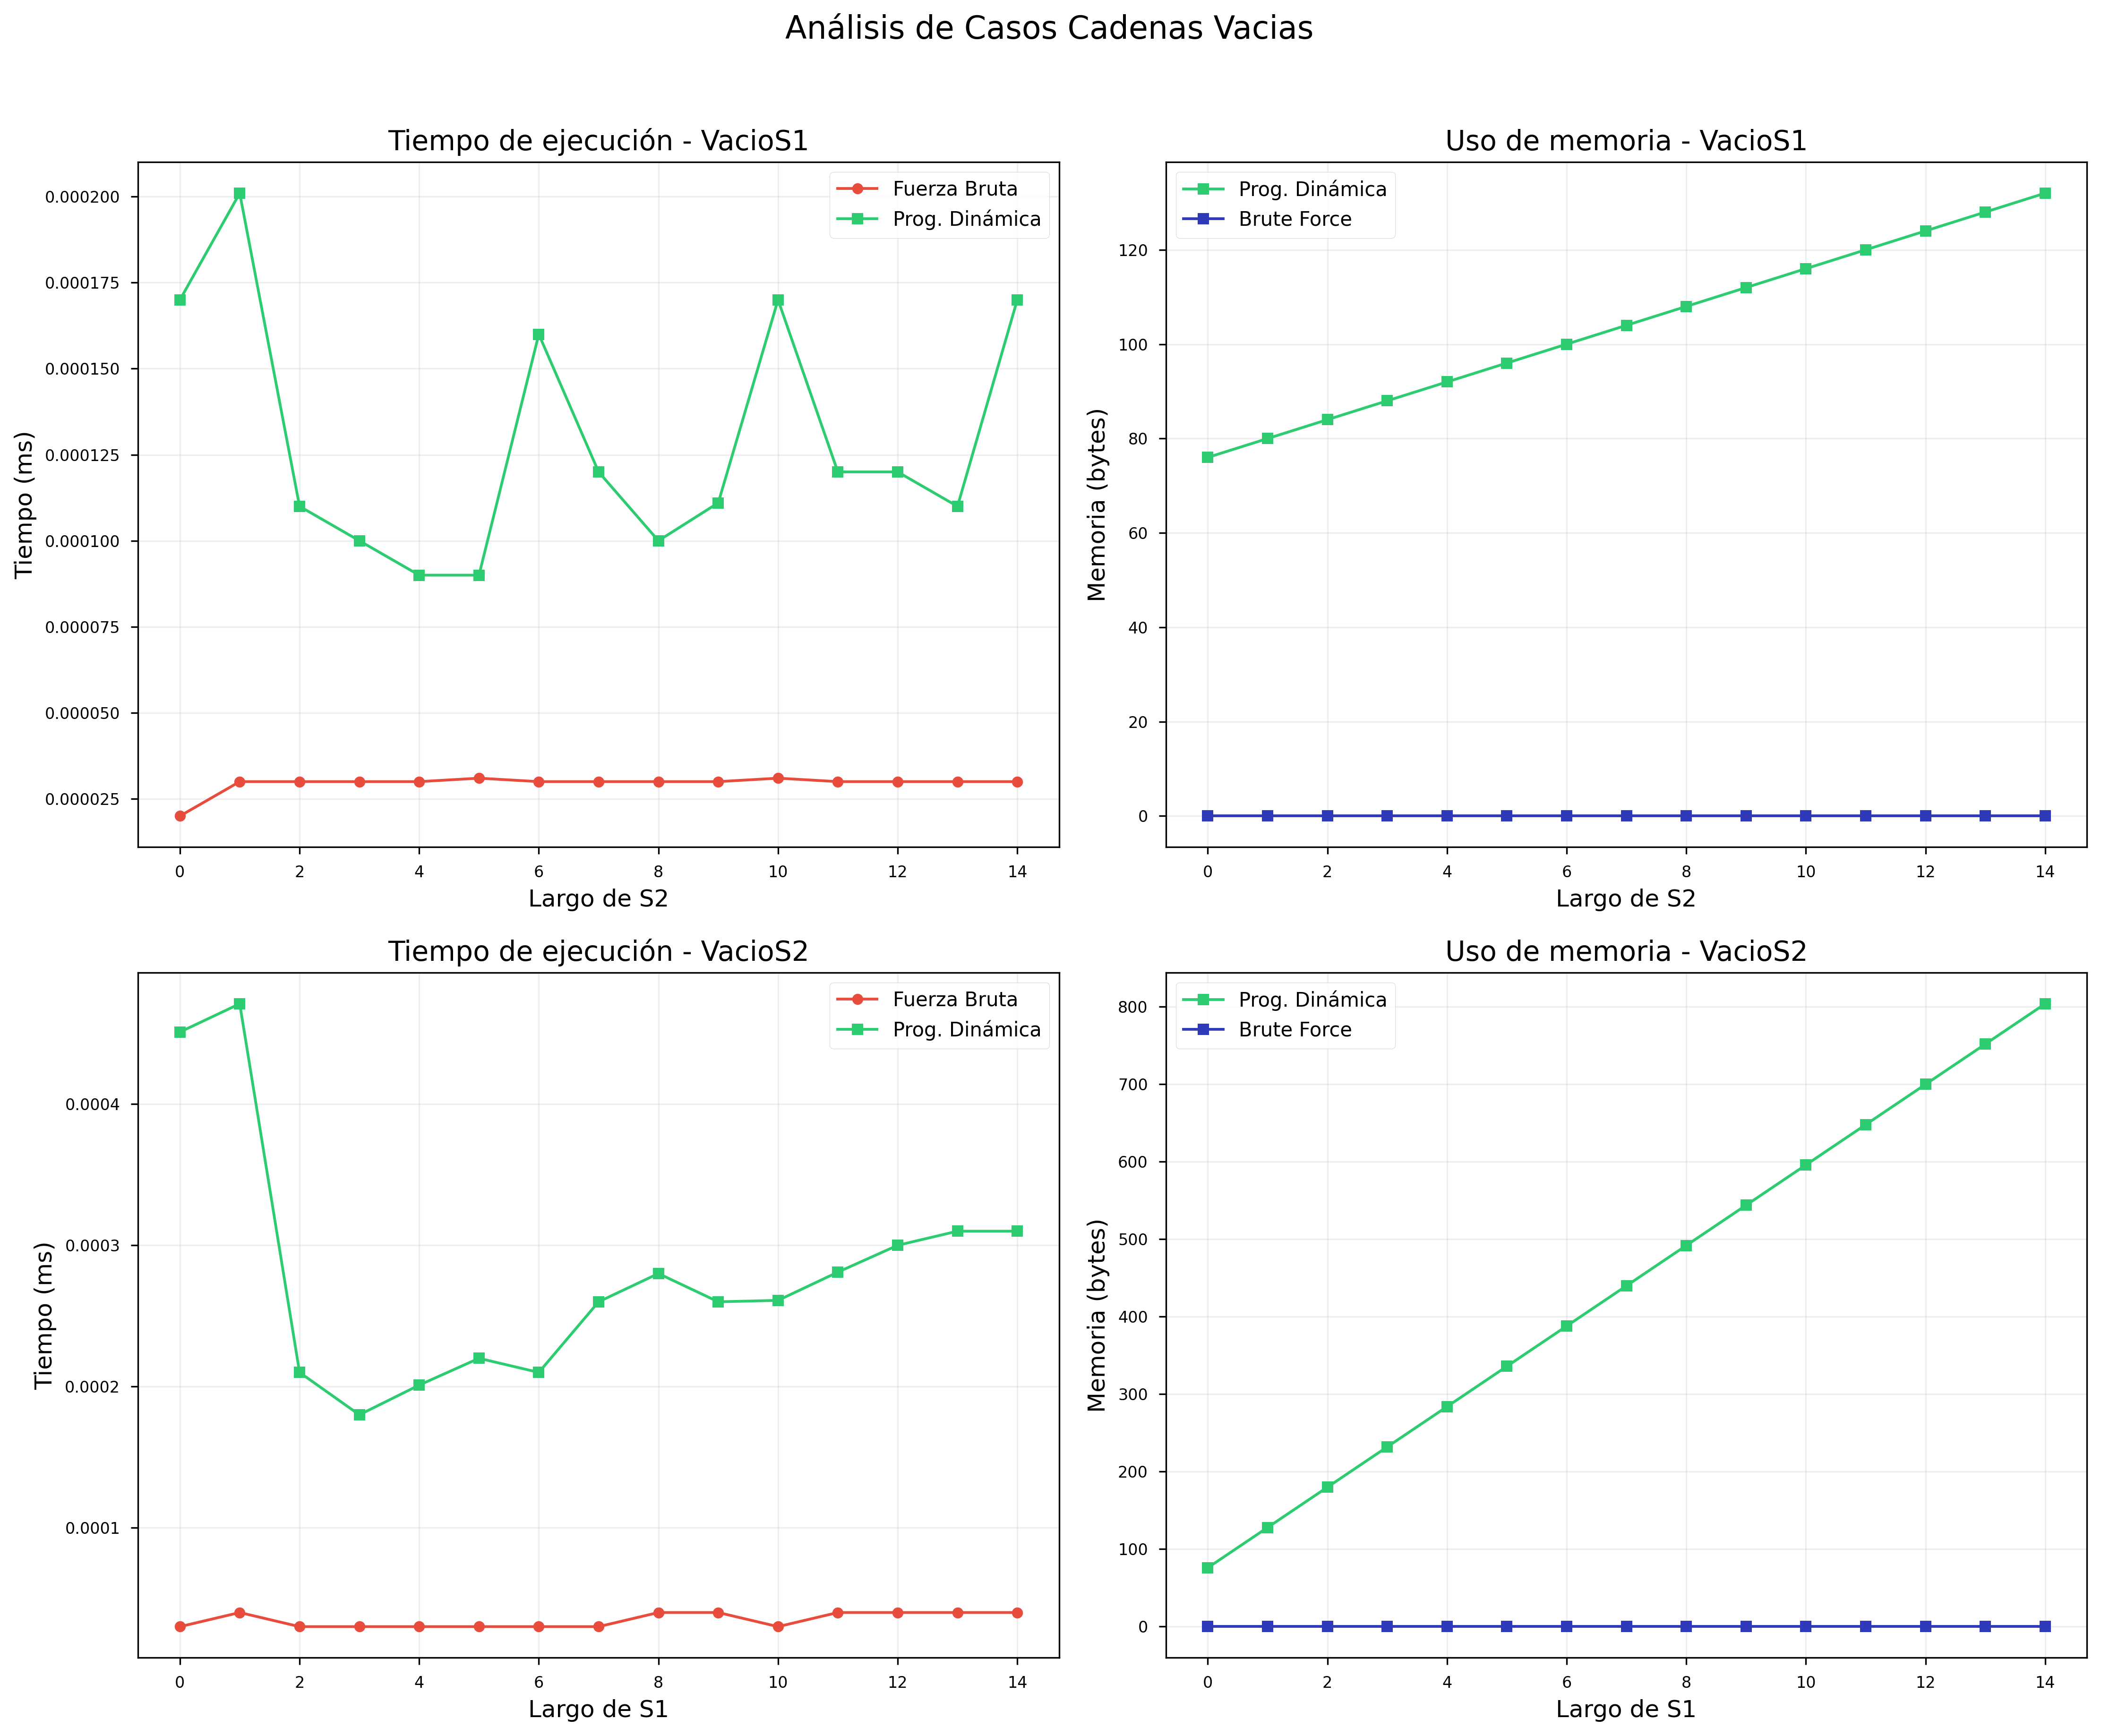
\includegraphics[width=\textwidth]{images/casos_especiales.png} 
        \caption{Casos Cadenas Vacias}
    \label{fig:scatterplot_5}
\end{figure}
Las cadenas vacias representan el mejor caso para fuerza bruta, ya que realiza trabajo lineal en vez de exponencial, por esta misma razon le gana en tiempo de ejecucion
a programacion dinamica.
\begin{figure}[H]
    \centering
        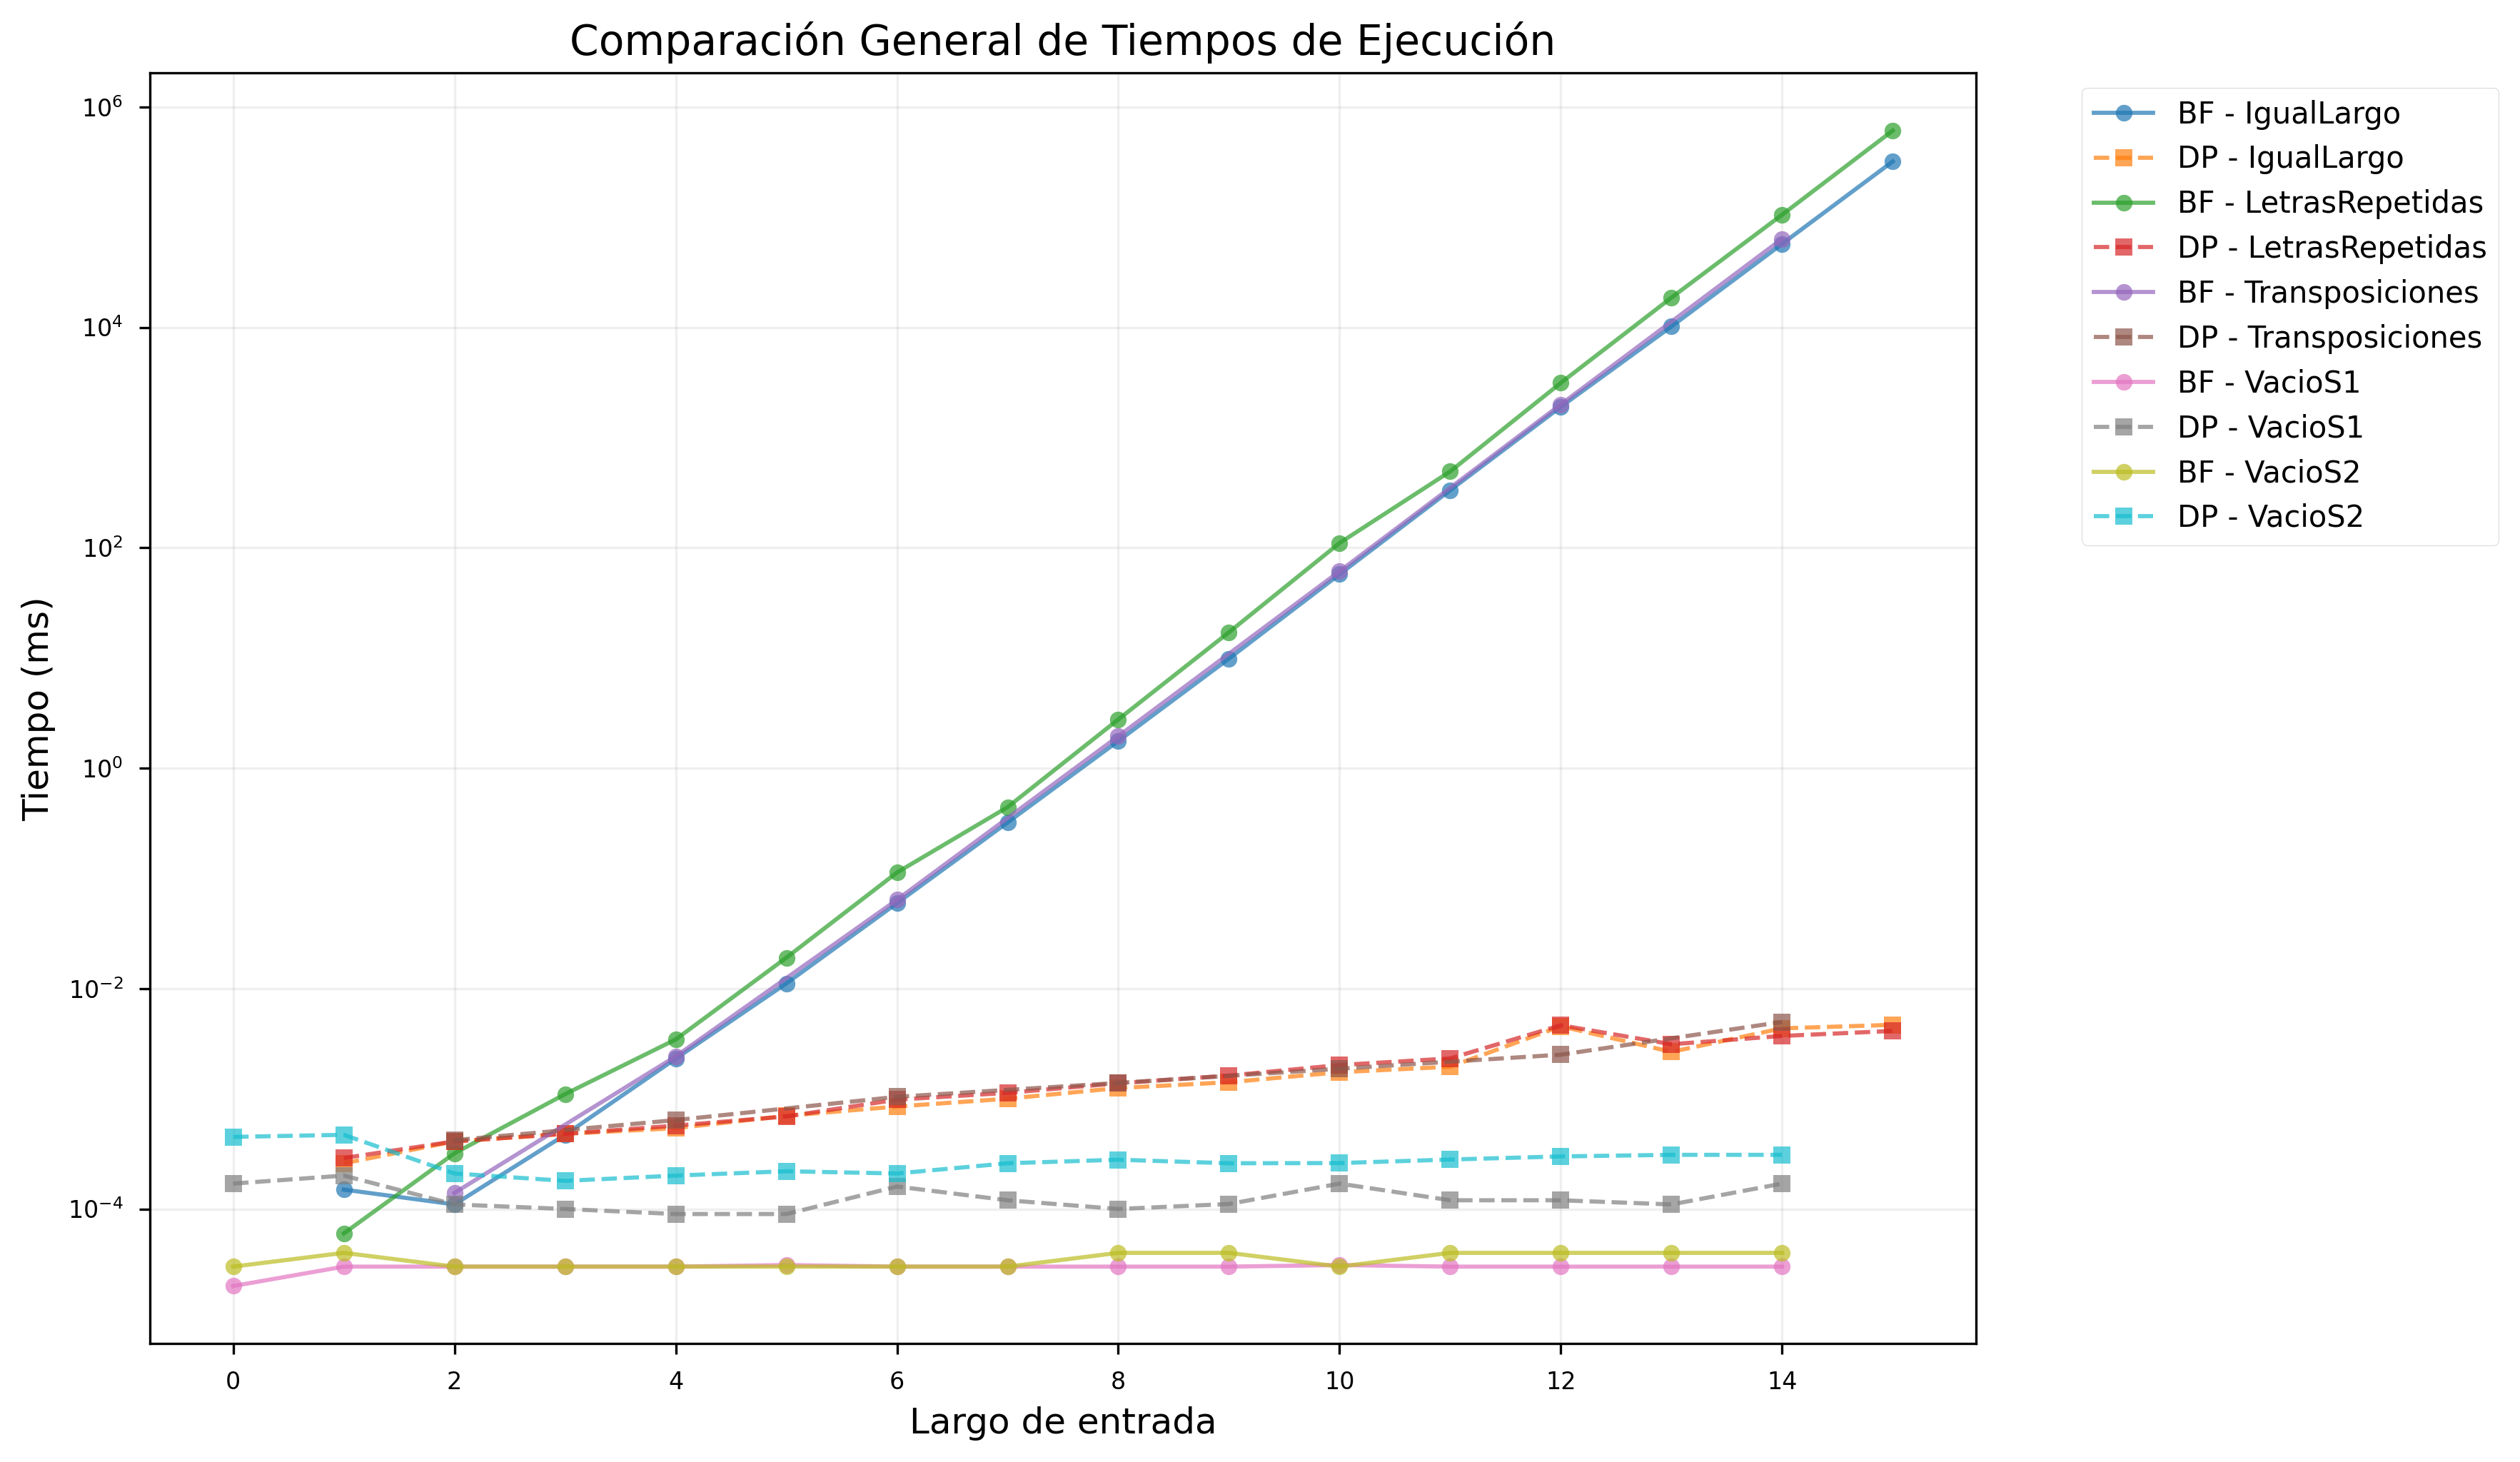
\includegraphics[width=\textwidth]{images/comparacion_general_tiempos.png}    
    \caption{Resumen general de resultados}
    \label{fig:scatterplot_6}
\end{figure}
Finalmente si queremos resolver el problema de la menor distancia, es importante tener en cuenta que el enfoque de fuerza bruta para cadenas vacias 
puede llegar a ser util, sin embargo el enfoque de programacion dinamica es una buena opcion general
